% !TeX root = _main.tex
% ROLE 2 -- DU LIEU, MO HINH, KIEM CHUNG, AS-IS, MO HINH MO RONG (muc 5--7).
% Nguoi nhan: nhom tu dien. Muc tieu: 5--7 trang noi dung chinh.
% DUOC SUA: file nay, figures/r2_*; nhan \label bat dau bang r2:.
% analysis/ do role 2 dau moi quan ly; bao role 3 truoc khi sinh lai dau ra.
% DAU VAO: analysis/run_analysis.py, extension_analysis.py, data/run_log.txt, data/ext_run_log.txt.
% BAN GIAO: tham so co don vi va nguon, kiem chung, AS-IS, dinh vi 2/5, du bao hoc may.

\section{Dữ liệu, giả định và phương pháp phân tích}
\label{r2:method}
\subsection{Nguồn dữ liệu và hiệu chỉnh quy mô}
Nhóm chưa có dữ liệu giao dịch của một cửa hàng cụ thể. Vì vậy \textbf{lượt xe
đến được mô phỏng}, nhưng \textbf{quy mô và các tham số chính được hiệu chỉnh
từ số liệu công bố} và ghi rõ loại căn cứ: R (số liệu công bố), E (ước tính
nhóm suy ra từ số liệu công bố), G (giả định cần đo lại). Chuỗi suy luận như sau:
\begin{equation}
\frac{110\,000\ \text{m}^3/\text{tháng}\times1000}{453\ \text{cửa hàng}\times30\ \text{ngày}}
\approx 8\,094\ \text{lít/cửa hàng/ngày}\quad\text{(R)}.
\end{equation}
Với khoảng 5,6 triệu xe máy và mức tiêu thụ 0,5 lít/xe/ngày, xe máy dùng khoảng
84\,000~m$^3$/tháng, tức 75\% lượng xăng (E). Một lượt xe máy đổ 2,5 lít (bình
4,4--5,2 lít~\cite{tank}, đổ khi còn khoảng một nửa), một lượt ô tô 30 lít (E).
Từ đó cửa hàng đại diện có $8\,094\times0{,}75/2{,}5\approx2\,428$ lượt xe máy
và $8\,094\times0{,}25/30\approx67$ lượt ô tô mỗi ngày; ô tô chỉ chiếm 2,7\%
số lượt. Mã \texttt{run\_analysis.py} tính lại toàn bộ chuỗi này và ghi vào
\path{data/run_log.txt}~\cite{analysis}.

\begin{table}[htbp]\centering\small
\caption{Tham số đầu vào, đơn vị và căn cứ (R: công bố; E: ước tính từ số liệu công bố; G: giả định)}\label{r2:assumptions}
\begin{tabularx}{\linewidth}{@{}p{38mm}p{37mm}p{6mm}Y@{}}
\toprule
Tham số & Giá trị (đơn vị) & Loại & Căn cứ / cách đo lại \\
\midrule
Lượng xăng bán / cửa hàng & 8\,094 lít/ngày & R & 110\,000 m$^3$/tháng; 453 cửa hàng~\cite{sct2026} \\
Lượt xe / ngày & 2\,495 xe/ngày (xe máy 2\,428; ô tô 67) & E & Chia theo số lít/lượt; đo lại bằng hóa đơn điện tử \\
Phân bố theo giờ $\lambda_t$ & 112--225 xe/giờ, đỉnh 18--19 giờ & G & Hai đỉnh đi làm/tan tầm; đo bằng dấu thời gian hóa đơn \\
$E[S]$ AS-IS & xe máy 1,5; ô tô 4,0 phút/xe (bình quân 1,57) & G & Tài liệu: 1--4 phút/xe máy~\cite{batui}; bấm giờ mẫu \\
$E[S]$ TO-BE & giảm 20\% (bình quân 1,25 phút/xe) & G & Trả trước QR/ứng dụng; đã thử trường hợp chỉ giảm 10\% \\
Hệ số biến thiên $S$ & CV = 0,8 & G & Lognormal; kiểm tra bằng dữ liệu bấm giờ \\
Số vòi / nhân viên AS-IS & 8 vòi; 6 nhân viên mỗi giờ & G & Cửa hàng nội thành điển hình \\
Ngưỡng bỏ đi & 20 xe đang chờ ($\approx$2,5--3 xe/vòi) & G & Quan sát số xe bỏ đi khi hàng dài \\
Chi phí nhân viên & 58\,000 đồng/giờ & E & 10 triệu đồng/tháng~\cite{wage} $\times$1,215 (BHXH) / 208 giờ \\
Lãi gộp bán lẻ & 1\,500 đồng/lít & E & Chiết khấu thực tế 100--2\,600 đồng/lít~\cite{chietkhau} \\
Chi phí số hóa & 250\,000 đồng/ngày & G & Ứng dụng trả trước, QR, tích hợp POS \\
Mục tiêu dịch vụ & $E[W_q]\le2$ phút; $P(W_q{>}5)\le5\%$ & G & Nhóm đặt; khách bỏ đi $\le1\%$ \\
\bottomrule
\end{tabularx}
\end{table}

\subsection{Định nghĩa chỉ số và đơn vị}
Với lượt xe $i$, gọi $a_i$, $b_i$, $d_i$ là thời điểm vào hàng chờ, bắt đầu
được phục vụ và rời trụ (phút, Hình~\ref{r1:bpmn}):
\begin{equation}
 w_{q,i}=b_i-a_i,\qquad s_i=d_i-b_i,\qquad w_i=d_i-a_i.
\end{equation}
Báo cáo dùng $\overline{W_q}$, phân vị 90\% $W_q^{90}$, tỷ lệ
$P(W_q{>}5)=N^{-1}\sum_i\mathbf 1(w_{q,i}>5)$ (tính trên xe đã vào hàng), tỷ
lệ bỏ đi (xe đến nhưng không vào hàng vì đã có từ 20 xe chờ), $W_q$ theo loại
xe, giờ nhân viên/ngày và chi phí (nghìn đồng/ngày).

\subsection{Mô hình hàng đợi M/M/c để tham chiếu}
Giả định dòng đến Poisson, thời gian phục vụ phân phối mũ, $c$ kênh giống nhau,
FCFS. Đặt $\lambda$ (xe/giờ), $\mu=60/E[S]$ (xe/giờ/kênh), $a=\lambda/\mu$,
$\rho=\lambda/(c\mu)<1$:
\begin{align}
 P_0&=\left[\sum_{n=0}^{c-1}\frac{a^n}{n!}+\frac{a^c}{c!(1-\rho)}\right]^{-1},\qquad
 C(c,a)=\frac{a^c}{c!(1-\rho)}P_0,\\
 E[W_q]&=\frac{60\,C(c,a)}{c\mu-\lambda}\ \text{(phút)},\qquad
 P(W_q>t)=C(c,a)\,e^{-(c\mu-\lambda)t/60}\ \ (t\text{ phút}).
\end{align}
Theo định luật Little, $L_q=\lambda E[W_q]/60$ (xe). Với $E[S]=1{,}57$ phút,
$\mu=38{,}3$ xe/giờ/kênh. Tính riêng từng giờ là xấp xỉ trạng thái ổn định.
\todo{2}{Bổ sung trích dẫn giáo trình/bài giảng L4 cho Erlang C và Little.}

\subsection{Mô phỏng sự kiện rời rạc}
Mỗi giờ sinh số xe theo Poisson với $\lambda_t$, thời điểm đến đều trong giờ;
mỗi xe là ô tô với xác suất 2,7\%. Thời gian phục vụ lấy mẫu lognormal theo
loại xe (CV = 0,8). Khi số xe đang chờ đã từ 20 trở lên, xe mới đến bỏ đi.
Số kênh đổi theo giờ; kênh đang phục vụ hoàn tất xe hiện tại khi giảm ca.
M/M/c dùng để chọn số kênh sơ bộ; mô phỏng dùng để đánh giá hai loại xe, CV
khác 1 và hành vi bỏ đi mà công thức không mô tả.

\section{Kiểm chứng và phân tích hiện trạng}
\label{r2:diagnosis}
\subsection{Kiểm tra dữ liệu đầu vào}
Bộ AS-IS có 50\,144 lượt xe trong 20 ngày mô phỏng; $E[S]=1{,}568$ phút, CV
0,86 (gồm cả trộn hai loại xe), khớp tham số sinh dữ liệu. Đây là kiểm tra
tính nhất quán nội bộ, không thay cho dữ liệu đo thực.
\begin{figure}[htbp]\centering
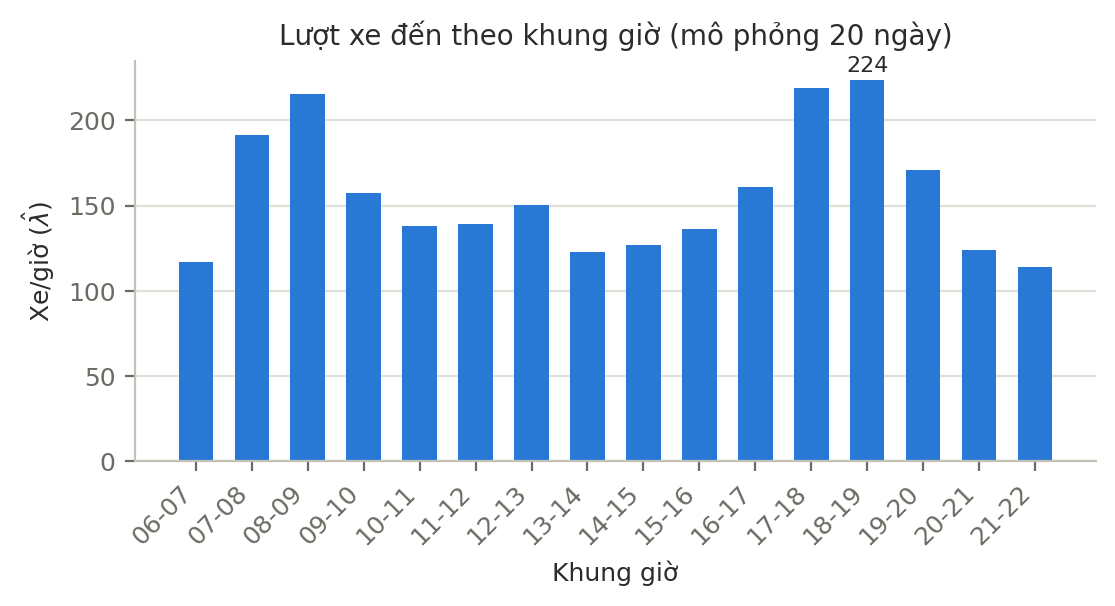
\includegraphics[width=0.9\linewidth]{figures/fig_arrivals.png}
\caption{Lượt xe đến theo khung giờ trong dữ liệu mô phỏng.}\label{r2:arrivals}
\source{\texttt{analysis/run\_analysis.py}; dữ liệu mô phỏng}
\end{figure}
\resulttable{tab_lambda.tex}{Lượt xe đến theo giờ và tham số sinh dữ liệu}{r2:lambda}
\FloatBarrier

\subsection{Đối chiếu công thức và mô phỏng}
\resulttable{tab_validation.tex}{Đối chiếu M/M/c với mô phỏng CV = 1, một loại xe, FCFS, 40 ngày/cấu hình, không bỏ đi}{r2:validation}
Ở $\rho\le0{,}84$, sai lệch nằm trong khoảng $-7{,}4\%$ đến $+7{,}5\%$. Ở
$\rho=0{,}98$ ($\lambda=225$, $c=6$) công thức cho 12,17 phút còn mô phỏng
7,61 phút ($-37{,}5\%$): khi gần bão hòa, mỗi ngày bắt đầu với hàng rỗng và
một giờ không đủ để hệ đạt trạng thái ổn định. Cấu hình $\lambda=212$, $c=5$
có $\rho=1{,}11$, không ổn định. Do đó M/M/c chỉ dùng để chọn công suất; kết
luận về phương án dựa trên mô phỏng.

\subsection{Điểm nghẽn AS-IS}
\resulttable{tab_asis_hourly.tex}{M/M/c theo giờ với 6 kênh và $E[S]=1{,}57$ phút}{r2:hourly}
\begin{figure}[htbp]\centering
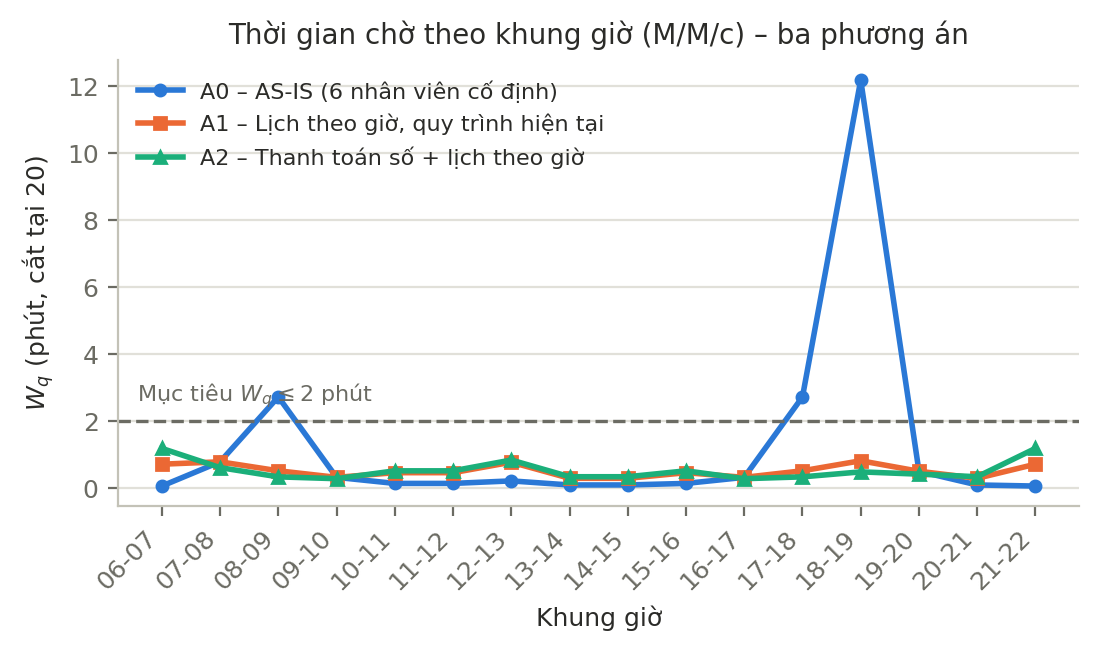
\includegraphics[width=0.89\linewidth]{figures/fig_wq_by_hour.png}
\caption{Thời gian chờ M/M/c theo giờ của ba phương án.}\label{r2:wq-hour}
\source{\texttt{analysis/run\_analysis.py}; tham số Bảng~\ref{r2:assumptions}}
\end{figure}
Lịch cố định 6 nhân viên vừa \emph{thừa} vừa \emph{thiếu}. Từ 09:00 đến 17:00,
$\rho$ chỉ 0,54--0,71; trong khi giờ 18--19 có $\rho=0{,}98$, $E[W_q]=12{,}17$
phút và 64\% xe chờ quá 5 phút; hai giờ 08--09 và 17--18 cũng vượt mục tiêu
(18,3\% chờ quá 5 phút). Mô phỏng cả ngày cho kết quả trung bình ``đẹp'' ---
$\overline{W_q}=0{,}64$ phút, mức sử dụng 67,9\% --- nhưng trong giờ 17--19
có 6,2\% xe chờ quá 5 phút và 2,3\% xe bỏ đi. Chẩn đoán vì vậy phải xét theo
giờ, không theo trung bình ngày.
\todo{2}{Thay $\lambda_t$ giả định bằng số hóa đơn điện tử theo giờ của một cửa
hàng thật (tối thiểu 4 tuần) và chạy lại toàn bộ.}

\section{Mô hình mở rộng: định vị rời rạc và dự báo nhu cầu}
\label{r2:extension}
\subsection{Chọn 2 trong 5 điểm mở cửa hàng mới}
\label{r2:location}
\textbf{Bài toán.} Doanh nghiệp có ngân sách mở $k=2$ cửa hàng mới và đã khảo
sát 5 vị trí ứng viên $J$ trên các trục chính; nhu cầu đến từ 8 quận $I$.
Bài toán định vị phân bố được rời rạc hóa bằng hai tập này. Dân số lấy theo
Tổng điều tra 2019~\cite{census2019}; nhu cầu mà một cửa hàng mới có thể thu
hút ở vùng $i$ là
\begin{equation}
h_i=\text{dân số}_i\times0{,}695\ \tfrac{\text{xe}}{\text{người}}\times0{,}2\
\tfrac{\text{lượt}}{\text{xe}\cdot\text{ngày}}\times2\%\ \text{(thị phần)},
\end{equation}
với 0,695 = 5,6 triệu xe máy / 8,05 triệu dân (E), 0,2 lượt/ngày = đổ 2,5 lít
mỗi 5 ngày (E), thị phần 2\% (G). Thời gian đi lại $t_{ij}$ (phút) tính từ tọa
độ xấp xỉ: khoảng cách đường chim bay $\times1{,}35$ (hệ số đường vòng), tốc
độ 20~km/giờ giờ cao điểm, cộng 2 phút ra/vào. Ngưỡng tiếp cận $R=15$ phút.
Năng lực một cửa hàng 8 vòi là $Q_j=2\,889$ lượt/ngày: giờ cao điểm (9\% lượt
ngày) tối đa 260 xe/giờ để vẫn đạt $\rho\le0{,}85$, $W_q\le2$ phút. Chi phí cố
định $f_j$ (thuê đất, khấu hao, quản lý) là 120, 150, 80, 95, 75 triệu đồng/tháng
cho J1--J5 (G). Mỗi lượt đóng góp $3{,}24\times1\,500-2\,165\approx2\,700$ đồng
(lãi gộp trừ lương nhân viên theo lượt).

\textbf{Mô hình.} $a_{ij}=1$ nếu $t_{ij}\le R$ (mã hóa nhị phân); vùng $i$ được
phủ khi tồn tại $j$ có $a_{ij}=1$ và $y_j=1$. Quyết định mở điểm được tích hợp
với phân bổ nhu cầu, chỉ giao cho điểm đã mở và không vượt năng lực:
\begin{align}
\text{(a)}\ \max\ \textstyle\sum_i h_i z_i \quad\text{hoặc}\quad
\text{(b)}\ \max\ 30\cdot2\,700\textstyle\sum_i h_i z_i/10^6-\sum_j f_j y_j \label{r2:mclp}\\
\text{với}\ \textstyle\sum_j y_j=2,\ x_{ij}\le a_{ij}y_j,\ \sum_j x_{ij}=z_i\le1,\
\sum_i h_i x_{ij}\le Q_j y_j,\ x,y,z\in\{0,1\}. \nonumber
\end{align}
Mục tiêu (a) là phục vụ được nhiều người nhất; mục tiêu (b) là lợi nhuận
(triệu đồng/tháng). Với $\binom52=10$ tổ hợp, nhóm liệt kê toàn bộ cách giao
vùng nên nghiệm là tối ưu chính xác.
\exttable{tab_ext_cover_matrix.tex}{Dân số, nhu cầu $h_i$ và thời gian đi lại $t_{ij}$ (phút); $^{\bullet}$ đánh dấu $a_{ij}=1$ ($t_{ij}\le15$ phút)}{r2:cover}
\exttable{tab_ext_location.tex}{Mười tổ hợp 2/5 điểm, xếp theo mục tiêu (a); lợi nhuận theo mục tiêu (b)}{r2:loc-result}
\begin{figure}[htbp]\centering
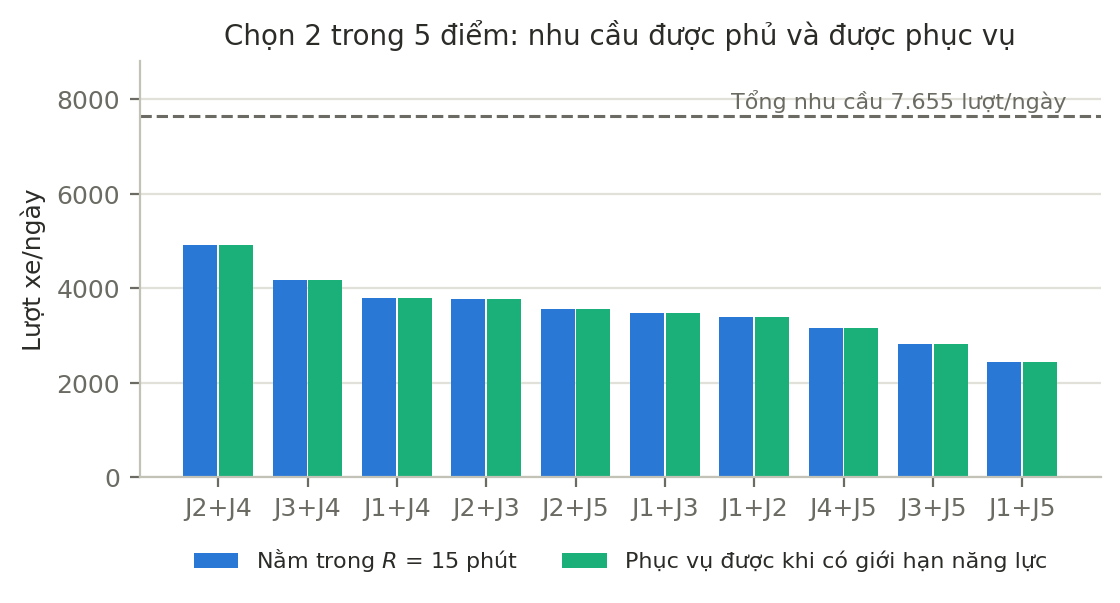
\includegraphics[width=0.9\linewidth]{figures/r2_location.png}
\caption{Nhu cầu nằm trong ngưỡng $R$ và nhu cầu phục vụ được của mười tổ hợp.}
\label{r2:loc-fig}
\source{\texttt{analysis/extension\_analysis.py}; dân số 2019, các tham số còn lại là ước tính/giả định}
\end{figure}

\textbf{Hai mục tiêu cho hai câu trả lời.} Theo mục tiêu (a), \textbf{J2 Đống Đa +
J4 Hoàng Mai} phục vụ 4\,916 lượt/ngày (64,2\% nhu cầu); J2 nhận Cầu Giấy, Đống
Đa, Thanh Xuân (2\,664 lượt/ngày, $\rho_{\max}=0{,}78$). Theo mục tiêu (b),
\textbf{J3 Hà Đông + J4 Hoàng Mai} lãi 163,2 triệu đồng/tháng so với 153,2 triệu
của J2 + J4, dù chỉ phục vụ 54,5\% nhu cầu: J2 nằm ở vùng giá thuê cao
(150 triệu đồng/tháng) và phải gánh tải gần năng lực. Một doanh nghiệp tư nhân
chịu áp lực chiết khấu thấp sẽ chọn (b); nếu mục tiêu là độ phủ dịch vụ (ví
dụ cam kết với đầu mối về sản lượng), (a) phù hợp hơn.

\exttable{tab_ext_location_sens.tex}{Độ nhạy của quyết định định vị}{r2:loc-sens}
\textbf{Độ bền.} J3 + J4 là tổ hợp lãi nhất ở 5/6 tình huống: $R=15$ hoặc 20
phút, nhu cầu giảm 20\% (KB-A), tăng 20\% (KB-B) và cửa hàng chỉ có 6 vòi; khi
nhu cầu tăng 20\%, J3 + J4 còn trở thành phương án phục vụ nhiều nhất vì J2 bị
giới hạn năng lực. Ngược lại, lợi nhuận của J2 + J4 giảm còn 73,6 triệu khi
nhu cầu giảm 20\% và còn 18,9 triệu nếu chỉ có 6 vòi. Chỉ khi $R=12$ phút (khách
rất ngại đi xa) thì tối ưu lợi nhuận chuyển sang J4 + J5. Kết luận BT2:
\textbf{chọn J3 Hà Đông + J4 Hoàng Mai}, giữ J4 cố định và coi J2/J3 là lựa
chọn phụ thuộc mục tiêu.
\todo{2}{Thay tọa độ xấp xỉ bằng địa chỉ ứng viên thật và thời gian đi lại từ
bản đồ số; kiểm tra lại số cửa hàng đối thủ trong bán kính $R$ để hiệu chỉnh thị phần 2\%.}

\subsection{Dự báo lượt xe ngày tới bằng học máy}
\label{r2:forecast}
Lịch theo giờ (BT1) chỉ tốt khi biết trước $\lambda_t$. Nhu cầu xăng có các
biến động \emph{biết trước được}: giá điều chỉnh vào 15 giờ thứ Năm hằng tuần
(tăng giá thì khách đổ trước 15 giờ, giảm giá thì chờ sau 15 giờ), tuần trước
Tết và kỳ nghỉ Tết, và tín hiệu căng thẳng nguồn cung. Nhóm dựng lịch sử 2 năm
(25/11/2024--22/11/2026) với \emph{lịch sự kiện thật}: Tết Ất Tỵ 29/1/2025, Tết
Bính Ngọ 17/2/2026, đợt cửa hàng đóng cửa giữa 2025 và đợt 17 cửa hàng tạm
dừng bán đầu tháng 3/2026~\cite{vtc2026}; biên độ điều chỉnh giá theo tuần lấy
quanh mức của các kỳ gần đây (1\,310--2\,075 đồng/lít~\cite{moit2026}). Lượt xe
trong lịch sử là mô phỏng. Mô hình học máy là hồi quy Poisson (GLM, ước lượng IRLS):
\begin{multline}
\log\lambda_{d,h}=\beta_h+\gamma_{\text{thứ}(d)}+\delta_1\sin\tfrac{2\pi d}{364}+\delta_2\cos\tfrac{2\pi d}{364}
+\tau_1 T^{\text{trước}}_d+\tau_2 T^{\text{nghỉ}}_d\\
+\pi_1\Delta p_d\mathbf 1_{h<15}+\pi_2\Delta p_d\mathbf 1_{h\ge15}+\pi_3\Delta p_{d-1}+\eta s_{d-1}+\kappa\ell_{d-1},
\end{multline}
với $\Delta p_d$ là mức điều chỉnh dự kiến (nghìn đồng/lít, tính được trước từ
giá thế giới), $s_{d-1}$ là tín hiệu nguồn cung hôm trước, $\ell_{d-1}$ là log tỷ
số lượt hôm trước so với trung bình 28 ngày. Học trên 23/12/2024--4/1/2026,
kiểm tra trên 84 ngày 5/1--29/3/2026 (có Tết và đợt tháng 3).
\exttable{tab_ext_ml_acc.tex}{Độ chính xác dự báo trên 84 ngày kiểm tra; ``ngày sự kiện'' là 25 ngày có Tết, điều chỉnh giá $\ge$1\,000 đồng/lít hoặc căng thẳng nguồn cung}{r2:ml-acc}
\begin{figure}[htbp]\centering
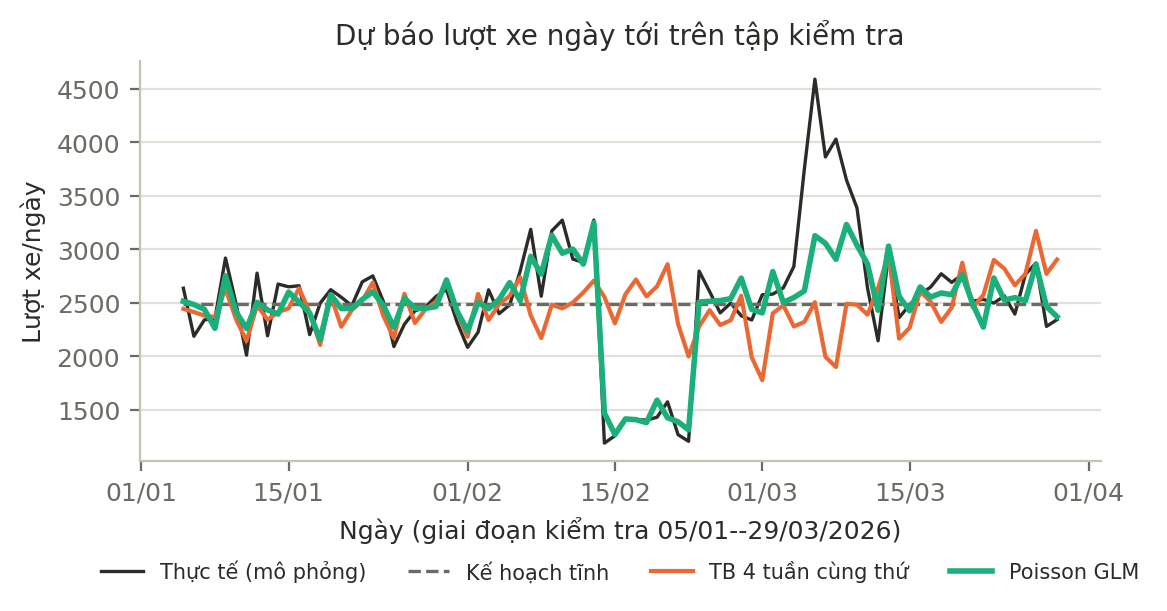
\includegraphics[width=0.9\linewidth]{figures/r2_forecast.png}
\caption{Dự báo tổng lượt xe/ngày trên tập kiểm tra.}\label{r2:ml-fig}
\source{\texttt{analysis/extension\_analysis.py}; lượt xe mô phỏng, lịch sự kiện theo thực tế}
\end{figure}
GLM giảm MAPE tổng ngày từ 18,33\% (kế hoạch tĩnh) và 19,63\% (trung bình 4 tuần
cùng thứ) xuống 7,25\%; trên 25 ngày sự kiện, từ khoảng 46\% xuống 10,44\%.
Trung bình 4 tuần thậm chí kém kế hoạch tĩnh vì nó ``nhớ'' Tết và đợt tháng 3
sang các tuần sau (Hình~\ref{r2:ml-fig}). Hệ số ước lượng có ý nghĩa vận hành:
tuần trước Tết $+18\%$ ($e^{0{,}167}$), kỳ nghỉ Tết $-42\%$ ($e^{-0{,}540}$), mỗi
nghìn đồng/lít tăng giá làm lượt xe trước 15 giờ tăng 28\% ($e^{0{,}249}$).
Giá trị vận hành của dự báo được đánh giá ở Mục~\ref{r3:ml-staff}.
\todo{2}{Huấn luyện lại trên dữ liệu hóa đơn điện tử thật; giữ cách chia theo
thời gian (không trộn ngẫu nhiên) và báo cáo MAPE theo tháng.}
